\documentclass[handout]{beamer}

\usetheme[progressbar=frametitle]{metropolis}
\metroset{block=fill}

\subtitle{NTIN071 Automata and Grammars}
\author{Jakub Bulín (KTIML MFF UK)}

\date{Spring 2025\\ 
    \vspace{1in} 
    \begin{flushleft}
        \it \footnotesize * Adapted from the Czech-lecture slides by Marta Vomlelová with gratitude. The translation, some modifications, and all errors are mine.
    \end{flushleft}
}

%% packages

\usepackage{amsmath}
\usepackage{amssymb}
\usepackage{amsthm}
\usepackage{cancel}
\usepackage{color}
\usepackage{colortbl}
\usepackage{forest}
\usepackage[utf8x]{inputenc}
\usepackage{multicol}
\usepackage{multirow}

%% colors
\definecolor{Gray}{gray}{0.9}

%% TikZ
\usepackage{tikz}
    \usetikzlibrary{
        automata,
        arrows,
        backgrounds,
        decorations.pathmorphing,
        fit,
        positioning,
        shapes,
        shapes.geometric,
        tikzmark
    } 
    \tikzset{>=stealth',shorten >=1pt,auto,node distance=2cm}
    \tikzset{initial text={}}
    \tikzset{elliptic state/.style={draw,ellipse}}

%% amsthm
\theoremstyle{plain}
    \newtheorem*{algorithm}{Algorithm}    
    \newtheorem*{observation}{Observation}
    \newtheorem*{proposition}{Proposition}

\theoremstyle{remark}
    \newtheorem*{exercise}{Exercise}
    \newtheorem*{remark}{Remark}

%% macros
\DeclareMathOperator{\RegE}{RegE}
\DeclareMathOperator{\RL}{RL}

% Just for Lecture 2
\newcommand{\x}{$\times$}
\newcommand{\nx}{\ }



\title{Lecture 12 -- Undecidable problems, Post's correspondence problem}


\begin{document}


\frame{\titlepage}


\begin{frame}{Recap of Lecture 11}
	
    \begin{itemize}        
        \item Recursively enumerable languages are exactly those generated by (Type 0) grammars
        \begin{itemize}
            \item TM to G: simulate moves on a reversed non-terminal copy of $\omega$, generate sufficient space, cleanup if accepting state
            \item G to TM: generate all strings, check if any of them represents a valid derivation of $\omega$ (sentential forms separated by $\#$)
        \end{itemize}   
        \item Context-sensitive languages:
        \begin{itemize}
            \item context-sensitive grammars are equivalent to monotone grammars
            \item Linear Bounded Automaton (LBA): nondeterministic TM with tape limited to the length of input
            \item constructions: monotone grammar to LBA, LBA to monotone grammar
        \end{itemize}
        \item Intro to computability: an overview
        \item decision problem $\leftrightsquigarrow$ the language of all `YES' instances
        \item machine-readable encoding of TMs
    \end{itemize}
	
\end{frame}


\begin{frame}{The Diagonal language}
    
    Let \alert{$\mathrm{decode}(w)$} be the TM $M$ such that $\mathrm{code}(M)=w$. (Recall: if $w$ is not a valid code, then $\mathrm{decode}(w)$ is a fixed one-state TM with no instructions.) Then:
    $$
    \alert{L_D}=\{w\mid w\notin L(\mathrm{decode}(w))\}
    $$
        
    \begin{theorem}
        $L_D$ is not recursively enumerable.
    \end{theorem}
    
    \textbf{Proof idea:} there cannot exist a TM recognizing $L_D$: running it on its own code would lead to Barber's paradox

    \bigskip

    \begin{quote}
        ``The program accepts all programs that don't accept themselves. Does the program accept itself?''
    \end{quote}

\end{frame}


\begin{frame}{Proof that $L_D=\{w\mid w\notin L(\mathrm{decode}(w))\}$ is not RE}

    \textbf{Proof:} Assume for contradiction that $L_D=L(M)$ for some $M$. Let $w=\mathrm{code}(M)$. Then $L_D=\{w\mid w\notin L(M)\}$. Is $w\in L(M)$?
    $$
    w\in L(M)\ \Leftrightarrow\ w\in L_D\ \Leftrightarrow\ w\notin L(M)
    $$
    
    \vspace{-24pt}
    \hfill\qedsymbol

    Why `diagonal'? A variant of Cantor's diagonal argument. Order all TMs by  $M_i=\mathrm{decode}(w_i)$. Does $M_i$ accept $w_j$?

    \vspace{-12pt}
    \begin{center}
        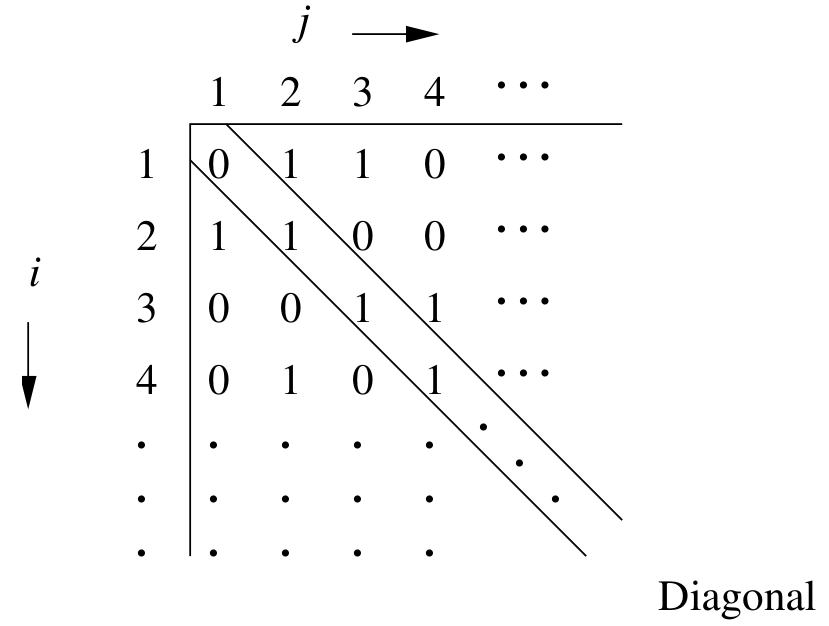
\includegraphics[width=0.48\textwidth]{files/diagonal.PNG}
    \end{center}
    \vspace{-15pt}
    A TM for $L_D$ would be one of the rows but differs from each row in the diagonal element. (Same as the proof that $\mathbb R$ is uncountable.)  
    
\end{frame}


\begin{frame}{The Universal Turing Machine}

    The \alert{Universal Turing Machine} $U$ can simulate any TM (given by its code) on any input. More precisely, $U$ accepts exactly inputs of the form \alert{$\langle \mathrm{code}(M),w\rangle$} where \alert{$w\in L(M)$}.
       
    \begin{columns}

        \column{0.5\textwidth}
        
        \textbf{The construction:}  four tapes
        \begin{enumerate}
            \item input tape ($w$ and the encoded transitions of $M$)
            \item simulated tape of $M$, symbols encoded as $0^i$, separated by 1s
            \item state of $M$, again represented by $0^i$
            \item scratch tape
        \end{enumerate}
    
        \column{0.5\textwidth}

        \begin{center}
            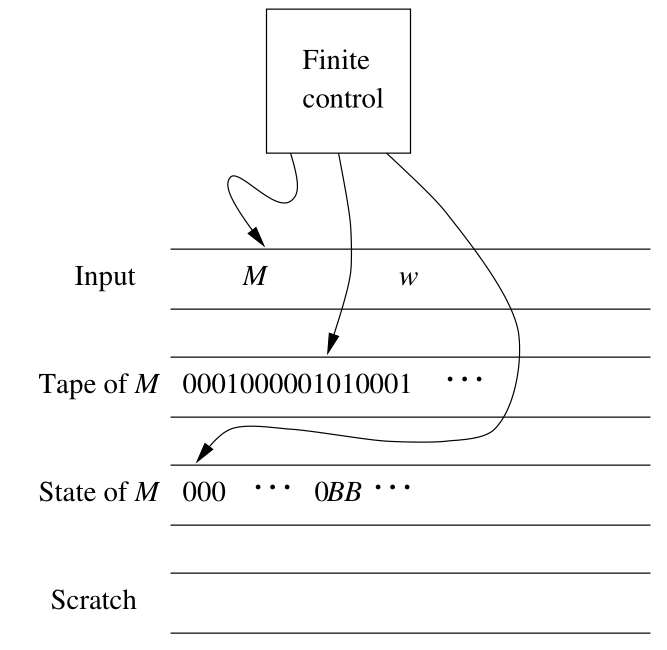
\includegraphics[width=\textwidth]{files/universalTM.PNG}
        \end{center}        
        
    \end{columns}

\end{frame}


\begin{frame}{The operation of $U$}

    \small
    \vspace{-3pt}
    \textbf{Initialize:}
    \vspace{-9pt}
    \begin{itemize}
        \item Check if the input code is valid, if not, halt without accepting
        \item Initialize Tape 2 with $w$ in its encoded form: $10$ for $0$ in $w$, $100$ for $1$\\ 
        Blanks are left blank and replaced with $1000$ only `on demand'\\ 
        Move 2nd head to the first simulated cell. 
        \item Place $0$ (the start state of $M$) on Tape 3.
    \end{itemize}
    \vspace{-3pt}
    \textbf{Simulate moves of $M$:}
    \vspace{-9pt}
    \begin{itemize}
            \item Search Tape 1 for the appropriate transition $0^i10^j10^k10^\ell10^m$, where $0^i$ on Tape 3, $0^j$ on Tape 2.
            \item Change the content of Tape 3 to $0^k$.
            \item Replace $0^j$ on Tape 2 by $0^\ell$. Scratch tape to manage spacing.
            \item Move head on Tape 2 to the next $1$ left or right, depending on $m$.
    \end{itemize}
    \vspace{-3pt}
    \textbf{Termination:} If $M$ has no transition matching simulated state \& tape symbol, halt without accepting. If $M$ enters accepting state, $U$ accepts.

\end{frame}


\begin{frame}{Recursive languages are closed under complement}

    \begin{lemma}
        If $L$ is recursive, then $\overline{L}$ is recursive as well.
    \end{lemma}

    \begin{center}
        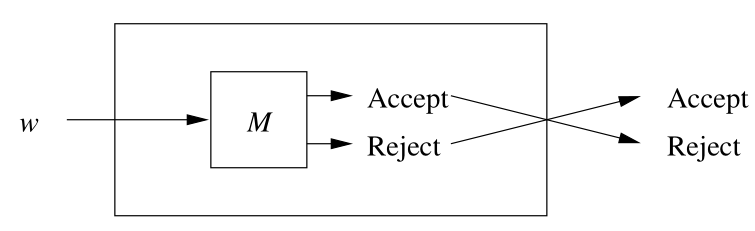
\includegraphics[width=0.7\textwidth]{files/compRec.PNG}
    \end{center}

    \textbf{Proof:} Given $M$ deciding $L$, construct $M'$ deciding $L'$. Since $M$ always halts, if it does not accept, the reason is missing transition. 
    
    \medskip $M'$ has a single, new accepting state $q_\text{ACCEPT}$. For every non-accepting state of $M$ and every tape symbol $X$ such that $\delta(q,X)$ is undefined, redefine $\delta'(q,X)=(q_\text{ACCEPT},X,L)$. 
    

    Clearly, $L(M')=\overline{L}$. Since $M$ is guaranteed to halt, so is $M'$.\hfill\qedsymbol    

\end{frame}


\begin{frame}{Post's theorem}

    \begin{theorem}
        $L$ is recursive iff both $L$ and $\overline{L}$ are recursively enumerable.
    \end{theorem}
    \vspace{-6pt}
    \textbf{Proof:} \alert{$\Rightarrow$} Follows from the lemma.
    \\ \alert{$\Leftarrow$} Let $L=L(M_1)$ and $\overline{L}=L(M_2)$. For an input $w$, simulate both $M_1$ and $M_2$ (two tapes, states with two components). $L$ and $\overline{L}$ are complementary, one of $M_1$ or $M_2$ will halt and accept.

    \vspace{-3pt}
    \begin{itemize}
        \item If $M_1$ accepts, accept.
        \item If $M_2$ accepts, reject.\hfill\qedsymbol
    \end{itemize}

    \vspace{-6pt}
    \begin{center}
        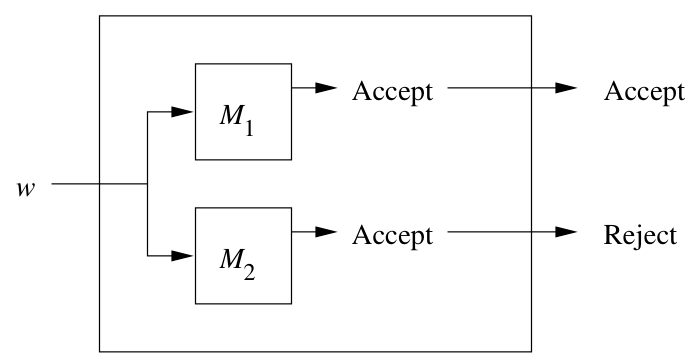
\includegraphics[width=0.6\textwidth]{files/bothRE.PNG}
    \end{center}

\end{frame}


\begin{frame}{The Universal language and its undecidability}

    $L_U=\{\langle \mathrm{code}(M),w\rangle\mid w\in L(M)\}$\hfill RE but not R\\
    $\overline{L_D}=\{w\mid w\in L(\mathrm{decode}(w))\}$\hfill RE but not R\\
    $L_D=\{w\mid w\notin L(\mathrm{decode}(w))\}$\hfill not RE

    \medskip

    \begin{theorem}
        The Universal language is recursively enumerable but not recursive. Same is true for complement of the Diagonal language.
    \end{theorem}    

    \vspace{-6pt}
    \textbf{Proof:}
    \vspace{-6pt}
        \begin{itemize}
            \item \alert{$L_U$ is RE:} it is recognized by the Universal TM $U$
            \item \alert{$\overline{L_D}$ is RE:} rewrite input $w$ to $\langle w,w\rangle=w111w$, then run on $U$
            \item \alert{$\overline{L_D}$ is not recursive:} if it were, by Post's theorem $L_D$ would be RE (actually R), but we know it is not
            \item \alert{$L_U$ is not recursive:} if it were, $\overline{L_D}$ would be recursive (rewrite $w$ to $\langle w,w\rangle$, run on the hypothetical $M$ deciding $L_U$)\hfill\qedsymbol
        \end{itemize}

\end{frame}


\begin{frame}{Reductions between decision problems}

    \begin{definition}
        A \alert{reduction} $R$ is an algorithm mapping all instances of $P_1$ to instances of $P_2$ that always halts, and for every instance $w$ of $P_1$ outputs an instance $R(w)$ of $P_2$ such that:
        \begin{itemize}
            \item $w$ is a YES instance of $P_1$ iff $R(W)$ is a YES instance of $P_2$
            \item $w$ is a NO instance of $P_1$ iff $R(W)$ is a NO instance of $P_2$
        \end{itemize}
        (Technically, $R=f_M$ for some TM $M$ that always halts.)
    \end{definition}
    
    \textbf{Example} The mapping $w\rightsquigarrow \langle w,w\rangle=w111w$ (from the previous proof) can clearly be done algorithmically. It is a reduction from $\overline{L_D}$ to $L_U$ (and also from $L_D$ to $\overline{L_U}$).

\end{frame}


\begin{frame}{Only easy reduce to easy, hard only reduce to hard}

    \begin{theorem}
        If there is a reduction from $P_1$ to $P_2$, then:
        \begin{enumerate}[(i)]            
            \item If $P_1$ is not decidable then neither is $P_2$.
            \item If $P_2$ is decidable, then so is $P_1$.
            \item If $P_1$ is not partially decidable then neither is $P_2$. 
            \item If $P_2$ is partially decidable, then so is $P_1$.
        \end{enumerate}
    \end{theorem}

    %\textbf{Proof:}
    \begin{itemize}
        \item[(i\&ii)] Let $P_1$ be undecidable. If $P_2$ were decidable, we could combine the reduction from $P_1$ to $P_2$ with the algorithm deciding $P_2$ to construct an algorithm that decides $P_1$.
        \item[(iii\&iv)] Assume $P_1$ is not partially decidable, but $P_2$ is. Similarly as above, we could combine the reduction and the algorithm for $P_2$ to get an algorithm partially deciding $P_1$--a contradiction.\hfill\qedsymbol
    \end{itemize}       

\end{frame}



\begin{frame}{``Does the given program halt for the given input?'}

    An instance of the \alert{Halting Problem} $\mathrm{Halt}$: $\langle \mathrm{code}(M),w\rangle\in \{0,1\}^*$. The answer is YES iff $M$ halts on input $w$; otherwise it is NO. 

    
    \begin{theorem}
        The Halting Problem is undecidable.
    \end{theorem}
    (Note that it is partially decidable: we can simulate using $U$.)

    \textbf{Proof:} Reduce the undecidable problem $\overline{L_D}$ to $\mathrm{Halt}$. Given an instance $w$ of $\overline{L_D}$, let $M=\mathrm{decode}(w)$. Modify $M$ to get $M'$ such that if $M$ \alert{halts without accepting}, $M'$ \alert{goes to an infinite loop}.

    Set \alert{$R(w)=\langle \mathrm{code}(M'),w\rangle$}. Clearly, it can be done algorithmically.

    \begin{itemize}
        \item If $w\in\overline{L_D}$, i.e. $w\in L(M)$, then $M'$ accepts (thus halts) on $w$.
        \item If $w\notin\overline{L_D}$, i.e. $w\notin L(M)$, then either $M$ doesn't halt or halts without accepting. In either case $M'$ doesn't halt on $w$. \hfill\qedsymbol
    \end{itemize}


\end{frame}


\begin{frame}{Accepts no inputs?}

    %Define the languages $L_e, L_{ne}\in \{0,1\}^*$ as follows:
    \begin{itemize}
        \item $L_e=\{\mathrm{code(M)}\mid L(M)=\emptyset\}$
        \item $L_{ne}=\{\mathrm{code(M)}\mid L(M)\neq\emptyset\}=\overline{L_e}$
    \end{itemize}

    \begin{theorem}
        \begin{enumerate}[(i)]
            \item $L_{e}$ is not recursively enumerable.
            \item $L_{ne}$ is recursively enumerable but not recursive.
        \end{enumerate}
    \end{theorem}

    \textbf{Proof:} As $L_{ne}=\overline{L_{e}}$, \alert{(i) follows from (ii)} by Post's theorem.

    \medskip

    \alert{$L_{ne}$ is RE:} nondeterministically guess $w\in L(M)$, verify using $U$
 
    \begin{center}
        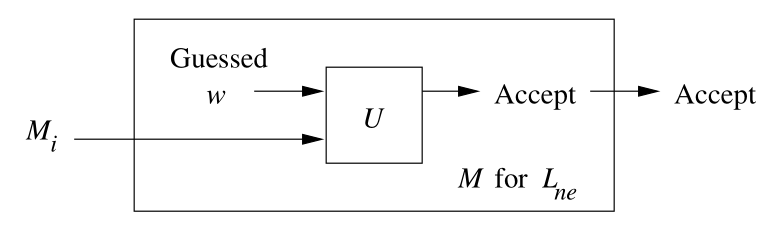
\includegraphics[width=0.8\textwidth]{files/Lne.PNG}
    \end{center}

\end{frame}


\begin{frame}{Proof cont'd}

    \alert{$L_{ne}$ is not recursive:} reduction from undecidable $\overline{L_D}$

    Given $w=\mathrm{code(M)}$, $R(w)$ is a TM $M'$ that ignores its input, rewrites the input tape with $w$, and simulates $M$ on $w$. 

    \begin{center}
        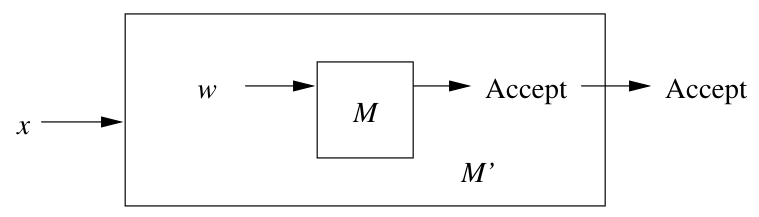
\includegraphics[width=0.8\textwidth]{files/Lne2.PNG}
    \end{center}
    
    \begin{itemize}
        \item If $w\in\overline{L_D}$, i.e. $w\in L(M)$, then $R(w)$ always accepts.
        \item If $w\notin\overline{L_D}$, i.e. $w\notin L(M)$, then $R(w)$ never accepts.\hfill\qedsymbol
    \end{itemize}

\end{frame}


\begin{frame}{Rice's theorem}

    Which properties of programs are decidable?

    \bigskip

    None of them!

    \bigskip

    (Except for trivial properties true/false for all programs.)

    \bigskip

    We have all the tools, but not the time to prove \href{https://en.wikipedia.org/wiki/Rice\%27s\_theorem}{\alert{Rice's theorem}}.

    \bigskip

    ``Theoretically, static analysis of programs cannot be done automatically?''

\end{frame}


\section*{Undecidable problems about context-free languages}


\begin{frame}{Post's correspondence problem}

    \vspace{-4pt}
    Several problems about context-free grammars are undecidable, e.g. is $L(G_1)\cap L(G_2)=\emptyset$? We show that by reduction from a suitable undecidable problem:
    
    \begin{block}{Post's correspondence problem (PCP)}
        \begin{itemize}
            \item \textbf{Instance:} two same-length lists of words over a finite alphabet $\Sigma$: \alert{$A=w_1,w_2,\ldots, w_k$}, \alert{$B=x_1,x_2,\ldots, x_k$}
            \item \textbf{Question:} is there a finite sequence of positive integers $i_1,\dots,i_m$ ($m\geq 1$) such that \alert{$w_{i_1} w_{i_2} \ldots w_{i_m}=x_{i_1} x_{i_2} \ldots x_{i_m}$}?
            \item call $i_1,\dots,i_m$ a \alert{solution}, $(w_i,x_i)$ a \alert{corresponding} pair
        \end{itemize}
    \end{block}
   
    %Note: indices in a solution can repeat!

    \begin{theorem}
        Post's correspondence problem is undecidable.
    \end{theorem}
    \vspace{-8pt}
    \textbf{Proof idea:} Reduction from $L_U$ by simulating computation of any TM on any input as a PCP instance. [detailes later, if there's time]

\end{frame}


\begin{frame}{Examples of PCP instances}

    \begin{columns}

        \column{0.68\textwidth}

        \textbf{Solvable instance:}

        \begin{itemize}            
            \item solution: \alert{$2,1,1,3$} (forms $101111110$)
            \item another solution: $2,1,1,3,2,1,1,3$
        \end{itemize}

        \smallskip

        \alert{partial solution}: $i_1,\dots,i_r$ such that one of $w_{i_1} \ldots w_{i_r}$, $x_{i_1} \ldots x_{i_r}$ is a prefix of the other

        \textbf{observe:} prefixes of solns are partial solns

        \column{0.32\textwidth}

        \begin{tabular}{c | l | l}
            & List $A$ & List $B$\\
           \hline
           $i$ & $w_i$ & $x_i$ \\
           \hline
           1 & 1 & 111\\
           2 & 10111 & 10\\
           3 & 10 & 0 
        \end{tabular}

        \vspace{0.5cm}
    
    \end{columns}

    \begin{columns}
    
        \column{0.65\textwidth}

        \textbf{Unsolvable instance:}

        \begin{itemize}
            \item $i_1=1$, $A:\textcolor{red}{10}$, $B:\textcolor{red}{10}\textcolor{blue}{1}$ (1st letter is 1)
            \item if $i_2=1$, $A:101\alert{0}$, $B:101\alert{1}01$
            \item if $i_2=2$, $A:10\alert{0}11$, $B:10\alert{1}11$
            \item so $i_2=3$, $A:\textcolor{red}{10101}$, $B:\textcolor{red}{10101}\textcolor{blue}{1}$
            \item same situation as after $i_1=1$, no way to get same length
        \end{itemize}

        \column{0.35\textwidth}

        \begin{tabular}{c | l | l}
            & List $A$ & List $B$\\
           \hline
           $i$ & $w_i$ & $x_i$ \\
           \hline
           1 & 10 & 101\\
           2 & 011 & 11\\
           3 & 101 & 011
        \end{tabular}
        
    \end{columns}

\end{frame}


\begin{frame}{Context-free languages and (un)decidability}

    Let $G,G'$ be context-free grammars, $R$ a regular expression, $\Sigma$ a finite alphabet, $w$ a word (all given on the input).

    \textbf{Recall}  that the following are \alert{decidable}:
    \begin{itemize}
        \item $L(G)\ni w$? [the CYK algorithm]
        \item $L(G)=\emptyset$? [check if $S$ is a generating symbol]
    \end{itemize}

    \medskip
    
    \begin{theorem}
        The following are \alert{undecidable}:

        \vspace{-9pt}
        \begin{enumerate}[(a)]
            \begin{multicols}{2}
                \item $L(G)=\Sigma^*$?
                \item $L(G)=L(R)$?
                \item $L(G)\supseteq L(R)$?
                \item $L(G)= L(G')$?
                \item $L(G)\supseteq L(G')$?
                \item $L(G)\cap L(G')\neq\emptyset$?
                \item Is $G$ ambiguous?
                \item[\phantom{(a)}] \phantom{Is $G$ ambiguous?}
            \end{multicols}
        \end{enumerate}    
    \end{theorem}
    \vspace{-9pt}
    We prove undecidability by reduction from the PCP problem.
        
\end{frame}


\begin{frame}{List languages}

    Given a PCP instance $(A=w_1,\ldots, w_k,B=x_1,\ldots, x_k)$, fix a set of new terminal symbols $S=\{s_1,\dots,s_k\}$ to represent indices.

    The \alert{list language $L_A$} for $A$ consists of all words of the form $w_{i_1}\dots w_{i_m}s_{i_m}\dots s_{i_1}$ where $m\geq 1$ and $i_j\in\{1,\dots,k\}$.

    \begin{itemize}
        \item $L_A$ is generated by $G_A=(\{A\},\Sigma\cup S,\mathcal P_A,A)$ with rules
        $$
        \mathcal P_A=\{A\to w_1 A a_1\mid\dots\mid w_k A a_k\mid w_1 a_1 \mid\dots\mid w_k a_k\}
        $$
        \item $L_A$ is recognized by a deterministic PDA (first store letters from $\Sigma$ on the stack, then for each $s_j$ pop $w_j^R$ from the stack)
        \item same is true for analogously defined \alert{$L_B$}
        \item the PCP instance $(A,B)$ has a solution iff $L_A\cap L_B\neq\emptyset$,
        \begin{align*}
            z&=w_{i_1}\dots w_{i_m}s_{i_m}\dots s_{i_1}\\
             &=x_{i_1}\dots x_{i_m}s_{i_m}\dots s_{i_1}\in L(A)\cap L(B)
        \end{align*}        

    \end{itemize}
    
\end{frame}


\begin{frame}{Proof of (g): Undecidability of ambiguiuty of $G$}

    \textbf{Recall:} ambiguous iff $\exists z\in L(G)$ with two different parse trees

    \medskip

    \alert{Reduction from PCP:} given $(A=w_1,\ldots, w_k,B=x_1,\ldots, x_k)$ construct $G=(\{S,A,B\},\Sigma\cup\{S\},\mathcal P,S)$ with rules
    \begin{minipage}{0.7\textwidth}
            
        \medskip
        $$
        \mathcal P=\{S\to A\mid B\}\cup\mathcal P_A\cup\mathcal P_B
        $$

        $G$ is ambiguous iff the PCP instance $(A,B)$ has a solution: Every $z\in L_A$ has a unique parse tree from $A$ (given by the $s_{i_j}$'s), same for $B$.
        
        \medskip
        
        Different parse trees for $z\in L(G)$ mean:
        \begin{itemize}
            \item $z=w_{i_1}\dots w_{i_m}s_{i_m}\dots s_{i_1}\in L_A$, and
            \item $z=x_{i_1}\dots x_{i_m}s_{i_m}\dots s_{i_1}\in L_B$, thus
            \item $z\in L_A\cap L_B$
        \end{itemize}
        Which happens iff $(A,B)$ has as solution.
    \end{minipage}
    \begin{minipage}{0.28\textwidth}
        \vspace{12pt}
        \scalebox{0.9}{
            \begin{forest}        
                [A [$w_{i_1}$][A [$w_{i_2}$][$\cdot$, edge={dotted} [A, edge=dotted [$w_{i_{m-1}}$][A [$w_{i_m}$][$s_{i_m}$]][$s_{i_{m-1}}$]]][$s_{i_2}$]][$s_{i_1}$]]
            \end{forest}
        }    

        \vspace{-18pt}
        \phantom{.}\hfill\qedsymbol
    \end{minipage}

\end{frame}


\begin{frame}{Proofs of (f), (a)} 

    \textbf{Proof of (f):} Undecidability of $L(G)\cap L(G')\neq\emptyset$

    \alert{Reduction from PCP:} the given PCP instance $(A,B)$ has a solution iff $L(G_A)\cap L(G_B)\neq\emptyset$\hfill\qedsymbol

    \textbf{Proof of (a):} Undecidability of $L(G)=\Sigma^*$

    Recall that $L_A,L_B$ are \alert{deterministic}. Since DCFLs are closed under complement, $L=\overline{L_A}\cup\overline{L_B}$ is context-free. Let $L=L(G)$. Then:
    
    \begin{center}
        $(A,B)$ has a solution $\ \Leftrightarrow\ $ $L_A\cap L_B\neq\emptyset$ $\ \Leftrightarrow\ $ $L(G)\neq(\Sigma\cup S)^*$\hfill\qedsymbol
    \end{center}

    \textbf{Note:} We proved undecidability of ``$L(G)\neq\Sigma^*$?''. Undecidability of ``$L(G)=\Sigma^*$?'' follows easily: they are almost complementary, except for `invalid inputs':
    \begin{itemize}
        \item Check if input is a valid encoding of $G$ and $\Sigma$, if not, reject.
        \item If it is valid, run algorithm for ``$\neq$'' and reverse its answer.
    \end{itemize}

\end{frame}


\begin{frame}{The rest of the proof is easy}
    
    \textbf{Proof of (b), (c):} Undecidability of $L(G)=L(R)$, $L(G)\supseteq L(R)$

    \alert{Reduction from $L(G)=\Sigma^*$}, create a regular expression $R$ such that $L(R)=\Sigma^*$

    \bigskip

    \textbf{Proof of (d), (e):} Undecidability of $L(G)= L(G')$, $L(G)\supseteq L(G')$

    \alert{Reduction from $L(G)=\Sigma^*$}, create a grammar $G'$ that generates all words in $\Sigma^*$
    \hfill\qedsymbol

    \bigskip

    \textbf{Note:} ``$L(G)\subseteq L(R)$?'' is decidable: 
    
    \vspace{-12pt}
    $$
    L(G)\subseteq L(R)\ \Leftrightarrow\ L(G)\cap \overline{L(R)}=\emptyset
    $$  

    and $L(G)\cap \overline{L(R)}$ is context-free (intersection with regular).

\end{frame}


\section*{Undecidability of Post's correspondence problem}

  
\begin{frame}{Modified Post's correspondence problem (MPCP)}
    
    A solution $(i_1,i_2,\dots,i_m)$ to a PCP instance $(A=w_1,\ldots, w_k,B=x_1,\ldots, x_k)$ is \alert{initial} if $i_1=1$, i.e., 
    $$
    {\bf w_1}w_{i_1} w_{i_2} \ldots w_{i_m}={\bf x_1}x_{i_1} x_{i_2} \ldots x_{i_m}
    $$
    
    \alert{Modified PCP}: Does a given PCP instance have an \alert{initial} solution?

       
    \textbf{Example:} This PCP instance has no initial solution:

    \begin{center}
        \small
        \begin{tabular}{c | l | l}
            & $A$ & $B$\\
            \hline
            $i$ & $w_i$ & $x_i$ \\
            \hline
            1 & 1 & 111\\
            2 & 10111 & 10\\
            3 & 10 & 0 
        \end{tabular}
    \end{center}

    Why? A:1, B:111 $\rightsquigarrow$ A:11, B:111111 $\rightsquigarrow$ A:111, B:111111111
        
    The lengths wont't match. Other choices lead to mismatch.

\end{frame}


\begin{frame}{Reducing MPCP to PCP}

    From $(A,B)$ construct $(C,D)$ such that $(A,B)$ has an initial solution iff $(C,D)$ has a solution.

    \textbf{The construction:} Add new symbols $*,\$\notin \Sigma$. Define $y_i$ from $w_i$ by adding $*$ after each letter, and $z_i$ from $x_i$ adding $*$ before each letter ($1\leq i\leq k$). Define $y_0=*y_1,z_0=z_1,y_{k+1}=\$,z_{k+1}=*\$$.
    
    \textbf{Example:}

    \vspace{-20pt}
    \begin{center}\small
        \begin{tabular}{c | l | l || l | l}
             & List $A$ & List $B$ & List $C$ & List $D$\\
            \hline
            $i$ & $w_i$ & $x_i$ & $y_i$ & $z_i$ \\
            \hline
            0 & & & *1* & *1*1*1\\
            1 & 1 & 111 & 1* & *1*1*1\\
            2 & 10111 & 10 & 1*0*1*1*1* & *1*0\\
            3 & 10 & 0 & 1*0* & *0\\
            4 & & & \$ & *\$ 
        \end{tabular}
    \end{center}
    Clearly, $({i_1}, {i_2}, \ldots, {i_m})$ is an initial solution to $(A,B)$ iff $(0,{i_1}, {i_2}, \ldots, {i_m},k+1)$ is a solution to $(C,D)$.\hfill\qedsymbol

\end{frame}


\begin{frame}{Undecidability of MPCP}

    \alert{Reduction from  $L_U$:} Given a TM $M$ and input $w$, construct $(A,B)$. Assume $M$ never writes $B$ and never moves left of inital position.

    \begin{center}
        \begin{tabular}{l l || l}
            List $A$ & List $B$\\
            \hline\hline
            \# & \#$q_0w$\#\\
            \hline
            $X$ & $X$ & for all tape symbols $X\in \Gamma$\\
            \# & \#\\
            \hline
            $qX$ & $Yp$ & for $\delta(q,X)=(p,Y,R) $\\
            $ZqX$ & $pZY$ & for $\delta(q,X)=(p,Y,L)$, $Z \in \Gamma $ tape symbol\\
            $q\#$ & $Yp\#$ & for $\delta(q,B)=(p,Y,R)$\\
            $Zq\#$ & $pZY\#$ & for $\delta(q,B)=(p,Y,L)$, $Z \in \Gamma $ tape symbol\\
            \hline
            $XqY$ & $q$& $q\in F$ accepting state\\
            $Xq$ & $q$& $q\in F$\\
            $qY$ & $q$& $q\in F$\\
            $q\#\#$ & $q\#$& $q\in F$
        \end{tabular}
    \end{center}

\end{frame}


\begin{frame}{Example: $M,w\rightsquigarrow(A,B)$}

    \footnotesize

    $M=(\{q_1,q_2,q_3\},\{0,1\},\{0,1,B\},\delta,q_1,B,\{q_3\})$, input word $w=01$
    
    \begin{columns}

        \column{0.6\textwidth}

        \begin{center}
            \begin{tabular}{c | c |c| c }
            & $0$ & $1$ & $B$ \\
            \hline 
            $\to q_1$ & $(q_2,1,R)$& $(q_2,0,L)$&  $(q_2,1,L)$\\
            $q_2$ & $(q_3,0,L)$ & $(q_1,0,R)$& $(q_2,0,R)$\\
            $* q_3$ & -- & -- & -- 
            \end{tabular} 
        \end{center}

        \begin{tabular}{cc|c}
            List $A$ & List $B$ & source\\
            \hline
            $q_10$ & $1q_2$ & $\delta(q_1,0)=(q_2,1,R)$ \\
            $0q_11$ & $q_200$ & $\delta(q_1,1)=(q_2,0,L)$ \\
            $1q_11$ & $q_210$ & $\delta(q_1,1)=(q_2,0,L)$ \\
            $0q_1\#$ & $q_201\#$ & $\delta(q_1,B)=(q_2,1,L)$ \\
            $1q_1\#$ & $q_211\#$ & $\delta(q_1,B)=(q_2,1,L)$ \\
            $0q_20$ & $q_300$ & $\delta(q_2,0)=(q_3,0,L)$ \\
            $1q_20$ & $q_310$ & $\delta(q_2,0)=(q_3,0,L)$ \\
            $q_21$ & $0q_1$ & $\delta(q_2,1)=(q_1,0,R)$ \\
            $q_2\#$ & $0q_2\#$ & $\delta(q_2,B)=(q_2,0,R)$ \\
            \vdots
        \end{tabular}    
    
        \column{0.4\textwidth}
        
        \begin{tabular}{cc|}
            List $A$ & List $B$\\
            \hline
            \# & \#$q_101$\#\\
            0 & 0\\
            1 & 1\\
            \# & \#\\
            \hline
            $0q_30$ & $q_3$ \\
            $0q_31$ & $q_3$ \\
            $1q_30$ & $q_3$ \\
            $1q_31$ & $q_3$ \\
            $0q_3$ & $q_3$ \\
            $1q_3$ & $q_3$ \\
            $q_30$ & $q_3$ \\
            $q_31$ & $q_3$ \\
            \hline
            $q_3\#\#$ & $\#$\\
            \hline
        \end{tabular}
        
    \end{columns}
    
\end{frame}


\begin{frame}{MPCP simulating the TM}

    \small

    \begin{minipage}{0.65\textwidth}
        \begin{tabular}{c  c |c| c }
         & List $A$ & List $B$ & source\\
        \hline
         & {\cellcolor{blue} $q_10$} & \cellcolor{blue}$1q_2$ &  $\delta(q_1,0)=(q_2,1,R)$ \\
         & $0q_11$ & $q_200$ & $\delta(q_1,1)=(q_2,0,L)$ \\
         & $1q_11$ & $q_210$ & $\delta(q_1,1)=(q_2,0,L)$ \\
         & {\cellcolor{violet}$0q_1\#$} & \cellcolor{violet}$q_201\#$ & $\delta(q_1,B)=(q_2,1,L)$ \\
         & $1q_1\#$ & $q_211\#$ & $\delta(q_1,B)=(q_2,1,L)$ \\
         & $0q_20$ & $q_300$ & $\delta(q_2,0)=(q_3,0,L)$ \\
         & {\cellcolor{orange} $1q_20$} & \cellcolor{orange}$q_310$ & $\delta(q_2,0)=(q_3,0,L)$ \\
         & {\cellcolor{red}$q_21$} & \cellcolor{red}$0q_1$ & $\delta(q_2,1)=(q_1,0,R)$ \\
         & $q_2\#$ & $0q_2\#$ & $\delta(q_2,B)=(q_2,0,R)$ \\
        \hline
        \end{tabular}
        
        \begin{itemize}
            \item Accepting path of $M$: $q_101\vdash 1q_21 \vdash 10q_1 \vdash 1q_201 \vdash q_3101$
        \end{itemize}
        
    \end{minipage}
    \begin{minipage}{0.001\textwidth}
    \ \end{minipage}
    \begin{minipage}{0.32\textwidth}
        \begin{tabular}{c c |c c}
         & List $A$ & List $B$ & \\
        \hline
        & \# & \#$q_101$\#\\
        &\uncover<3->{\cellcolor{green}}0 & \cellcolor{green}0 &\\
        & \cellcolor{green}1 & \cellcolor{green}1 &\\
        & \cellcolor{green}\# & \cellcolor{green}\# &\\
        \hline
         & \cellcolor{cyan}$0q_30$ & \cellcolor{cyan}$q_3$ & \\
         & \cellcolor{cyan}$0q_31$ & \cellcolor{cyan}$q_3$ & \\
         & \cellcolor{cyan}$1q_30$ & \cellcolor{cyan}$q_3$ & \\
         & \cellcolor{cyan}$1q_31$ & \cellcolor{cyan}$q_3$ & \\
         & \cellcolor{cyan}$0q_3$ & \cellcolor{cyan}$q_3$ & \\
         & \cellcolor{cyan}$1q_3$ & \cellcolor{cyan}$q_3$ & \\
         & \cellcolor{cyan}$q_30$ & \cellcolor{cyan}$q_3$ & \\
         & \cellcolor{cyan}$q_31$ & \cellcolor{cyan}$q_3$ & \\
        \hline
         & $q_3\#\#$ & $\#$ & 
        \end{tabular} 
    \end{minipage}
    \begin{tabular}{ l  l }
        $A:$ & $\#\uncover<2->{\color{blue} q_10}\uncover<3->{\color{green} 1\# 1}\uncover<4->{\color{red}q_21} \uncover<5->{\color{green}\# 1}\uncover<6->{\color{violet}0q_1 \#}\uncover<7->{\color{orange}  1q_20}\uncover<8->{\color{green} 1 \# \color{cyan}q_31\color{green}01\#\color{cyan} q_30\color{green}1\#\color{cyan} q_31\color{green}\#}\uncover<9->{\color{black} q_3\#\#}
        $\\
        $B:$ & $\#q_101\#\uncover<2->{\color{blue}  1q_2}\uncover<3->{\color{green}  1\# 1}\uncover<4->{\color{red}0q_1}\uncover<5->{\color{green} \# 1}\uncover<6->{\color{violet}q_201 \#}\uncover<7->{\color{orange} q_310}\uncover<8->{\color{green}1\# \color{cyan}q_3\color{green}01\# \color{cyan}q_3\color{green}1\# \color{cyan}q_3\color{green}\#}\uncover<9->{\color{black}\#}
        $
    \end{tabular}

\end{frame}

    
\begin{frame}{Undecidability of PCP}
    
    \begin{theorem}
        Post's correspondence problem is undecidable.
    \end{theorem}    
    \textbf{Proof:} We have already shown that MPCP reduces to PCP. To show that $L_U$ reduces to MPCP, we must verify that:
    
    $M$ accepts $w$ $\ \alert{\Leftrightarrow}\ $ the constructed $(A,B)$ has an initial solution

    \alert{$\Rightarrow$} If $w\in L(M)$, start with the initial pair and simulate the computation of $M$ on input $w$.  

    \alert{$\Leftarrow $} Given an initial solution to $(A,B)$, there is a corresponding computation of $M$ on $w$:
    \vspace{-3pt}
    \begin{itemize}
        \item MPCP must start with the initial pair
        \item while $q\notin F$, rules for cleaning cannot be used
        \item the partial solution is of the form A:$x$,B:$xy$, i.e., $B$ is longer
        \item thus we must end in an accepting state\hfill\qedsymbol
    \end{itemize}

\end{frame}


\begin{frame}{Summary of Lecture 12}

    \begin{itemize}
        \item the Diagonal language $L_D$ is not recursively enumerable
        \item the Universal language $L_U$, the Universal TM: simulate any $M$ on any $w$
        \item recursive languages are closed under complement
        \item Post's theorem: $L$ recursive iff both $L,\overline{L}$ are RE
        \item $L_U$, $\overline{L_D}$ are recursively enumerable but not recursive
        \item reductions between decision problems
        \item the Halting problem is undecidable        
        \item (Rice's thm: nontriv. properties of programs are undecidable)
        \item Undecidable problems about context-free grammars
        \item Source of undecidability: Post's correspondence problem
    \end{itemize}

\end{frame}


\end{document}
